\documentclass[11pt]{article}
\usepackage{amsmath,amssymb,amsthm}
\usepackage{graphicx}
\usepackage{float}
\usepackage{tikz}
\usetikzlibrary{arrows, quotes, trees}
\usepackage[margin=1in]{geometry}
\usepackage{fancyhdr}
\setlength{\parindent}{0pt}
\setlength{\parskip}{5pt plus 1pt}
\setlength{\headheight}{13.6pt}
\newcommand\question[2]{\vspace{.25in}\hrule\textbf{#1: #2}\vspace{.5em}\hrule\vspace{.10in}}
\renewcommand\part[1]{\vspace{.10in}\textbf{(#1)}}
\pagestyle{fancyplain}
\lhead{\textbf{\NAME\ (\UID)}}
\chead{\textbf{HW\HWNUM}}
\rhead{CS 6350, \today}

\tikzstyle{block} = [rectangle, draw, fill=white!20,
    text width=3em, text centered, rounded corners, minimum height=2em]
\tikzstyle{line} = [draw, very thick, color=black!50, -latex']
\tikzstyle{leaf} = [circle, draw, fill=none, text width=1em, text centered, minimum height=1em]

\begin{document}\raggedright

\newcommand\NAME{Jake Pitkin}
\newcommand\UID{u0891770}
\newcommand\HWNUM{1}

\question{1}{Decision trees}

\emph{Note: Square nodes test for feature values and round leaf nodes specify the class labels.}

\part{1} Representing Boolean functions as decision trees.

\part{a} $(x_1 \lor x_2) \land x_3$

\hspace*{30 mm}\begin{tikzpicture}[
box/.style = {rectangle, draw, align=center},
level distance = 18mm,
level 1/.style = {sibling distance=66mm},
edge from parent/.style = {draw, -latex'},
edge from parent fork down
                        ]
\node [block] {$x_3$} 
	child { 
      node [leaf] {0} 
      edge from parent node[left] {0}  
	} 
    child { 
      node [block] {$x_1$} 
        child { 
          node [block] {$x_2$}
          child {
          	node [leaf] {0}
          	edge from parent node[left] {0}
          }
          child {
          	node [leaf] {1}
          	edge from parent node[right] {1}
          } 
          edge from parent node[left] {0} 
        }
        child {
        	node [leaf] {1}
        	edge from parent node[right] {1}
        }
        edge from parent node[right] {1}  
    }; 
\end{tikzpicture}

\part{b} $(x_1 \land x_2) \ xor\ (\neg x_1 \lor x_3)$

\hspace*{30 mm}\begin{tikzpicture}[
box/.style = {rectangle, draw, align=center},
level distance = 18mm,
level 1/.style = {sibling distance=66mm},
level 3/.style = {sibling distance = 40mm},
edge from parent/.style = {draw, -latex'},
edge from parent fork down
                        ]
\node [block] {$x_1$} 
	child { %level 2
      node [leaf] {1} 
      edge from parent node[left] {0}  
	} 
    child { %level 2
      node [block] {$x_2$} 
        child { %level 3
          node [block] {$x_3$}
          child { %level 4
          	node [leaf] {0}
          	edge from parent node[left] {0}
          }
          child { %level 4
          	node [leaf] {1}
          	edge from parent node[right] {1}
          } 
          edge from parent node[left] {0} 
        }
        child { %level 3
        	node [block] {$x_3$}
        	child { %level 4
        		node [leaf] {1}
        		edge from parent node[left] {0}
        	}
        	child { %level 4
        		node [leaf] {0}
        		edge from parent node [right] {1}
        	}
        	edge from parent node[right] {1}
        }
        edge from parent node[right] {1}  
    }; 
\end{tikzpicture}

\newpage
\part{c} The 2-of-3 function defined as follows: at least 2 of $\{x_1, x_2, x_3\}$ should be true for the \hspace*{13 mm} output to be true.

\hspace*{30 mm}\begin{tikzpicture}[
box/.style = {rectangle, draw, align=center},
level distance = 18mm,
level 1/.style = {sibling distance=66mm},
level 2/.style = {sibling distance=40mm},
level 3/.style = {sibling distance = 10mm},
edge from parent/.style = {draw, -latex'},
edge from parent fork down
                        ]
\node [block] {$x_1$} 
	child { %level 2
      node [block] {$x_2$}
      child { %level 3
      	node [leaf] {0}
      	edge from parent node[left] {0}
      }
      child { % level 3
      	node [block] {$x_3$}
      	child { %level 4
      		node[leaf] {0}
      		edge from parent node[left] {0}
      	}
      	child { %level 4
      		node[leaf] {1}
      		edge from parent node[right] {1}
      	}
      	edge from parent node[right] {1}
      }
      edge from parent node[left] {0}  
	} 
    child { %level 2
      node [block] {$x_2$} 
        child { %level 3
          node [block] {$x_3$}
          child { %level 4
          	node [leaf] {0}
          	edge from parent node[left] {0}
          }
          child { %level 4
          	node [leaf] {1}
          	edge from parent node[right] {1}
          } 
          edge from parent node[left] {0} 
        }
        child { %level 3
        	node [leaf] {1}
        	edge from parent node[right] {1}
        }
        edge from parent node[right] {1}  
    }; 
\end{tikzpicture}

\part{2} Pok\'{e}mon Go decision tree to determine whether a Pok\'{e}mon can be caught.

\part{a} There are 2 choices for Berry, 3 choices for Ball, 3 choices for Color, and 4 choices for type. This gives $2 * 3 * 3 * 4 = 72$ possible outputs. We are making a Boolean decision, so there are two ways to fill each of those 72 outputs giving $2^{72}$ possible functions.

\framebox[1.5\width]{$2^{72}$ possible functions} \par

\part{b} Entropy is defined as: $$H(S) = -p_+\log(p_+) - p_-\log(p_-)$$
The training set contains 16 examples, 8 of which result in a catch while the other 8 do not. 
$$H(Caught) = -\frac{8}{16}\log(\frac{8}{16})-\frac{8}{16}\log(\frac{8}{16}) = 1$$

\framebox[1.5\width]{$H(Caught) = 1$} \par
	
\part{c} Information gain is defined as:
$$Gain(S, A) = H(S)\  - \sum_{v\in Values(A)} \frac{|S_v|}{|S|} H(S_v)$$

Berry = Yes. 7 out of 16 examples. Caught = 6/7 - Not Caught = 1/7. $H(berry_{yes}) = 0.592$.
Berry = No. 9 out of 16 examples. Caught = 2/9 - Not Caught = 7/9. $H(berry_{no}) = 0.764$.
$$Gain(S, Berry) = 1 - ((\frac{7}{16})(0.592) + (\frac{9}{16})(0.764)) = 0.689$$

\framebox[1.5\width]{$Gain(S, Berry) = 0.311$} \par
\newpage

Ball = Pok\'{e}. 6 out of 16 examples. Caught = 1/6 - Not Caught = 5/6. $H(ball_{poke}) = 0.65$.

Ball = Great. 7 out of 16 examples. Caught = 4/7 - Not Caught = 3/7. $H(ball_{great}) = 0.985$.

Ball = Ultra. 3 out of 16 examples. Caught = 3/3 - Not Caught = 0/3. $H(ball_{ultra}) = 0$.
$$Gain(S, Ball) = 1 - ((\frac{6}{16})(0.65) + (\frac{7}{16})(0.985) + (\frac{3}{16})(0)) = 0.325$$

\framebox[1.5\width]{$Gain(S, Ball) = 0.325$} \par

Color = Green. 3 out of 16 examples. Caught = 2/3 - Not Caught = 1/3. $H(color_{green}) = 0.918$.

Color = Yellow. 7 out of 16 examples. Caught = 3/7 - Not Caught = 4/7. $H(color_{yellow}) = 0.985$.

Color = Red. 6 out of 16 examples. Caught = 3/6 - Not Caught = 3/6. $H(color_{red}) = 1$.
$$Gain(S, Color) = 1 - ((\frac{3}{16})(0.918) + (\frac{7}{16})(0.985) + (\frac{6}{16})(1)) = 0.022$$

\framebox[1.5\width]{$Gain(S, Color) = 0.022$} \par 

Type = Normal. 6 out of 16 examples. Caught = 3/6 - Not Caught = 3/6. $H(type_{normal}) = 1$.

Type = Water. 4 out of 16 examples. Caught = 2/4 - Not Caught = 2/4. $H(type_{water}) = 1$.

Type = flying. 4 out of 16 examples. Caught = 3/4 - Not Caught = 1/4. $H(type_{flying}) = 0.811$.

Type = psychic. 2 out of 16 examples. Caught = 0/2 - Not Caught = 2/2. $H(type_{psychic}) = 0$.

$$Gain(S, Type) = 1 - ((\frac{6}{16})(1) + (\frac{4}{16})(1) + (\frac{4}{16})(0.811) + (\frac{2}{16})(0)) = 0.172$$

\framebox[1.5\width]{$Gain(S, Type) = 0.172$} \par 

\part{d} When using the ID3 algorithm to create a decision tree, I would select the attribute Ball as the root of the tree.

\setlength{\fboxsep}{4pt}
\framebox[2.1\width]{Ball} \par 
\newpage
\part{e}
\hspace*{0 mm}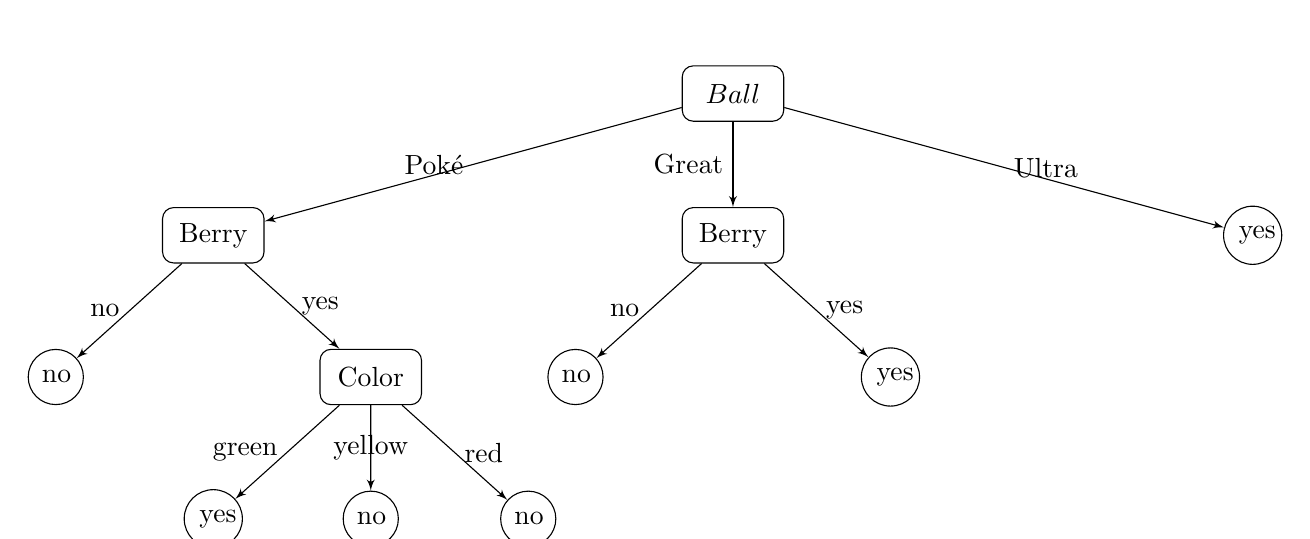
\begin{tikzpicture}[
box/.style = {rectangle, draw, align=center},
level distance = 18mm,
level 1/.style = {sibling distance=66mm},
level 2/.style = {sibling distance=40mm},
level 3/.style = {sibling distance = 20mm},
edge from parent/.style = {draw, -latex'},
%edge from parent fork down
                        ]
\node [block] {$Ball$} 
	child { %level 2
      node [block] {Berry}
      child { %level 3
      	node [leaf] {no}
      	edge from parent node[left] {no}
      }
      child { % level 3
      	node [block] {Color}
      	child { %level 4
      		node[leaf] {yes}
      		edge from parent node[left] {green}
      	}
      	child { %level 4
      		node[leaf] {no}
      		edge from parent node {yellow}
      	}
      	child { %level 4
      		node[leaf] {no}
      		edge from parent node[right] {red}
      	}
      	edge from parent node[right] {yes}
      }
      edge from parent node[left] {Pok\'{e}}  
	} 
	child { %level 2
		node [block] {Berry}
		child { %level 3
			node [leaf] {no}
			edge from parent node[left] {no}
		}
		child { %level 3
			node [leaf] {yes}
			edge from parent node[right] {yes}
		}
		edge from parent node [left]{Great}
	}
    child { %level 2
      node [leaf] {yes} 
      edge from parent node[right] {Ultra}  
    }; 
\end{tikzpicture}
 \quad Based on the common value for the attribute value $yellow$, a choice was made for the node \qquad Ball $\rightarrow$ Berry $\rightarrow$ Color. Across the training examples the most likely labeling is $no$.

\part{f}

\begin{table}[H]
\centering
\begin{tabular}{| c c c c | c | c |}
\hline
Berry& Ball & Color & Type & Caught & Correct Prediction?\\
\hline
Yes & Great & Yellow & Psychic & Yes & Yes \\
Yes & Pok\'e & Green & Flying & No & No \\
No & Ultra & Red & Water & No & No \\
\hline
\end{tabular}
\caption{Predictions for test set}
\end{table}

Out of the three examples in the test set, my decision tree predicted only one correct.

\framebox[1.5\width]{Accuracy = $33\%$} \par 

\part{g} I think using a decision tree to classify if a Pok\'{e}mon will be caught or not is a good idea. The training set provided is very sparse and I would expect a better rate of accuracy given more training data.

\part{3} Using the Gini measure with the ID3 algorithm.

\qquad \part{a} Information gain is defined as:
$$Gain(S, A) = Gini(S)\  - \sum_{v\in Values(A)} \frac{|S_v|}{|S|} Gini(S_v)$$

Caught = Yes. 8 out of 16 examples. Caught = No. 8 out of 16 examples. $Gini(S) = 0.5$ \newline

Berry = Yes. 7 out of 16 examples. Caught = 6/7 - Not Caught = 1/7. $Gini(berry_{yes}) = 0.245$.
 
Berry = No. 9 out of 16 examples. Caught = 2/9 - Not Caught = 7/9. $Gini(berry_{no}) = 0.346$.
$$Gain(S, Berry) = 0.5 - ((\frac{7}{16})(0.245) + (\frac{9}{16})(0.346)) = 0.2$$

\framebox[1.5\width]{$Gain(S, Berry) = 0.2$} \par

Ball = Pok\'{e}. 6 out of 16 examples. Caught = 1/6 - Not Caught = 5/6. $Gini(ball_{poke}) = 0.278$.

Ball = Great. 7 out of 16 examples. Caught = 4/7 - Not Caught = 3/7. $Gini(ball_{great}) = 0.49$.

Ball = Ultra. 3 out of 16 examples. Caught = 3/3 - Not Caught = 0/3. $Gini(ball_{ultra}) = 0$.
$$Gain(S, Ball) = 0.5 - ((\frac{6}{16})(0.278) + (\frac{7}{16})(0.49) + (\frac{3}{16})(0)) = 0.181$$

\framebox[1.5\width]{$Gain(S, Ball) = 0.181$} \par

Color = Green. 3 out of 16 examples. Caught = 2/3 - Not Caught = 1/3. $Gini(color_{green}) = 0.444$.

Color = Yellow. 7 out of 16 examples. Caught = 3/7 - Not Caught = 4/7. $Gini(color_{yellow}) = 0.49$.

Color = Red. 6 out of 16 examples. Caught = 3/6 - Not Caught = 3/6. $Gini(color_{red}) = 0.5$.
$$Gain(S, Color) = 0.5 - ((\frac{3}{16})(0.444) + (\frac{7}{16})(0.49) + (\frac{6}{16})(0.5)) = 0.015$$

\framebox[1.5\width]{$Gain(S, Color) = 0.015$} \par 

Type = Normal. 6 out of 16 examples. Caught = 3/6 - Not Caught = 3/6. $Gini(type_{normal}) = 0.5$.

Type = Water. 4 out of 16 examples. Caught = 2/4 - Not Caught = 2/4. $Gini(type_{water}) = 0.5$.

Type = flying. 4 out of 16 examples. Caught = 3/4 - Not Caught = 1/4. $Gini(type_{flying}) = 0.375$.

Type = psychic. 2 out of 16 examples. Caught = 0/2 - Not Caught = 2/2. $Gini(type_{psychic}) = 0$.

$$Gain(S, Type) = 0.5 - ((\frac{6}{16})(0.5) + (\frac{4}{16})(0.5) + (\frac{4}{16})(0.375) + (\frac{2}{16})(0)) = 0.094$$

\framebox[1.5\width]{$Gain(S, Type) = 0.094$} \par 



\qquad \part{b} I would pick Berry as the root of my decision tree. When using the Gini measure to calculate the information gain of each attribute, Berry has the highest information gain. This is different than when entropy is used to calculate information gain. When entropy is used, Ball is selected as the root.

\framebox[1.5\width]{Berry - different than when entropy is used}
\newpage
\question{2}{Linear Classifiers}

\part{1} Weights $\mathbf{w}$ and a bias $\mathbf{b}$ classifies the dataset from problem 1.
$$
\mathbf{w} = \begin{bmatrix}
0 \\
0 \\
1 \\
1 \\ 	
\end{bmatrix}
 and \ b = -1
$$
Looking at the dataset, one possible way to classify the data is either $x_3$ or $x_4$ must be set to produce an output of $1$. Otherwise, the output is $-1$.

\part{2} The table below details the accuracy of the linear classifier from part 1 on the dataset from part 2:
 \begin{center}
    \begin{tabular}{cccc|c|c}
      $x_1$ & $x_2$ & $x_3$ & $x_4$ & $o$ & $prediction$\\ \hline
      1 & 0 & 1 & 1 & 1 & 1\\
      0 & 1 & 0 & 1 & 1 & 1\\
      1 & 0 & 1 & 0 & 1 & 1\\
      1 & 1 & 0 & 0 & 1 & -1\\
      1 & 1 & 1 & 1 & 1 & 1\\
      1 & 1 & 1 & 0 & 1 & 1\\
      0 & 0 & 1 & 0 & -1 & 1\\
    \end{tabular}
  \end{center}
\framebox[1.5\width]{Accuracy = 5/7 or 71.4\%}

\part{3} Weights $\mathbf{w}$ and a bias $\mathbf{b}$ classifies the combined dataset from part 1, 2, and 3.
$$
\mathbf{w} = \begin{bmatrix}
1 \\
0 \\
0 \\
1 \\ 	
\end{bmatrix}
 and \ b = -1
$$
Looking at the combined dataset, we can see that either $x_1$ or $x_4$ must be set to produce an output of $1$. Otherwise, the output is $-1$.

\question{3}{Experiments}

\end{document}

